 \documentclass[12pt]{article}


 \usepackage[left=1in,top=1in,right=1in,bottom=1in]{geometry}

 %\renewcommand {\theequation}{\arabic{section}.\arabic{equation}}

 \usepackage{amsmath,amssymb,amsthm,amsfonts}
 %\usepackage{times}
 \usepackage{enumerate}
 \usepackage{epsfig}
 \usepackage{mdframed}
 \usepackage{pgf}
 \usepackage{tikz}
\usetikzlibrary{automata,positioning}
 \usepackage{pgfplots}
 \usepackage{blkarray}
 \usepackage[utf8]{inputenc}
\usepackage{natbib}
\usepackage{graphicx}
 

 
 \newtheorem{theorem}{Theorem}
 \newtheorem*{theorem*}{Theorem}
 \newtheorem{proposition}[theorem]{Proposition}
 \newtheorem{lemma}[theorem]{Lemma}
 \newtheorem{claim}[theorem]{Claim}
 \newtheorem{assumption}[theorem]{Assumption}
 \newtheorem{corollary}[theorem]{Corollary}
 \newtheorem*{corollary*}{Corollary}
 \newtheorem{conjecture}[theorem]{Conjecture}
 \newtheorem*{conjecture*}{Conjecture}

 \theoremstyle{remark}
 \newtheorem*{note}{Note}

 \newtheorem*{remark}{Remark}
 \newtheorem*{question}{Question}
 \newtheorem*{convention}{Convention}

 \theoremstyle{definition}
 \newtheorem{definition}[theorem]{Definition}
 \newtheorem*{fact}{Fact}
 \newtheorem{algorithm}{Algorithm}
 \newtheorem{example}[theorem]{Example}

 %numbering
 \numberwithin{figure}{section}
 %\numberwithin{equation}{section}


 \newcounter{fig}
 \newcommand{\ddt}{\frac{d}{dt}}
 \newcommand{\lskip}{\phantom{.}}
\newcommand{\red}[1]{\textcolor{red}{#1}}
 \newcommand{\RT}{\Rightarrow}
\newcommand{\tN}{\widetilde{N}}

 \def\R{\mathbb R}
 \def\Z{\mathbb Z}
 \def\C{\mathcal{C}}
 \def\S{\mathcal{S}}
 \def\Re{\mathcal{R}}
 \def\L{\mathbb{L}^V}
 \def\E{E}
 \def\F{\mathcal F}


 \newcommand{\eqdist}{\overset{\mathcal{D}}{=}}
 \newcommand{\eqdef}{\overset{\mbox{\tiny def}}{=}}

 \newcommand{\MT}{\mathcal{Z}}
 \newcommand{\ErrV}{\mathcal{E}^V}
 \newcommand{\Err}{\mathcal{E}}
 \newcommand{\cd}{\xrightarrow{d}}

 \newcommand{\EG}{\mathcal{A}}
 \newcommand{\TG}{\mathcal{B}}
 \newcommand{\EGV}{\mathcal{A}^V}
 \newcommand{\TGV}{\mathcal{B}^V}

 \newcommand{\noin}{\noindent}
 



 \begin{document}

 \tikzset{every node/.style={auto}}
 \tikzset{every state/.style={rectangle, minimum size=0pt, draw=none, font=\normalsize}}
 \tikzset{bend angle=20}
 \tikzset{
  loop above/.style={% original: above, out=105, in=75, loop
    above, in=45, out=135, loop,
    every loop/.append style={looseness=5}}}
 \tikzset{
  loop below/.style={% original: above, out=105, in=75, loop
    above, in=-45, out=225, loop,
    every loop/.append style={looseness=5}}}
 \tikzset{
  loop right/.style={% original: above, out=105, in=75, loop
    above, in=-45, out=45, loop,
    every loop/.append style={looseness=5}}}    
 \tikzset{
  loop left/.style={% original: above, out=105, in=75, loop
    above, in=135, out=225, loop,
    every loop/.append style={looseness=5}}}
    
    
 \begin{center}
 \textbf{\large \black{Homework 4}}
\end{center}

\begin{itemize}
  \item 
\textbf{Exercise 1.14.}\\
(a) \begin{center}
   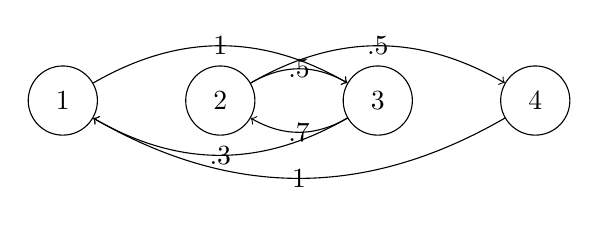
\begin{tikzpicture}[baseline={(current bounding box.center)}]
    %states
    \node[state] (2) at (-1,0) {$2$};
    \node[state] (3) at (1,0) {$3$};
    \node[state] (4) at (3,0) {$4$};
    \node[state] (1) at (-3,0) {$1$};
    %edges
    \path[->] 
%      (0) edge[loop above] node{$\frac{1}{3}$} (0)
     (1) edge[bend left] node{$1$} (3)
     (2) edge[bend left] node{$.5$} (3)
     (2) edge[bend left] node{$.5$} (4)
     (3) edge[bend left] node{$.3$} (1)
     (3) edge[bend left] node{$.7$} (2)
     (4) edge[bend left] node{$1$} (1);
   \end{tikzpicture} 
\end{center}
From the graph, we can know $\big\{1,2,3,4\big\}$ is an irreducible set, state $2$ is periodic with period $2$, by Lemma 68, we can know all states are periodic, thus, the chain \textbf{cannot} converge to equilibrium.\\
\\
(b) \begin{center}
   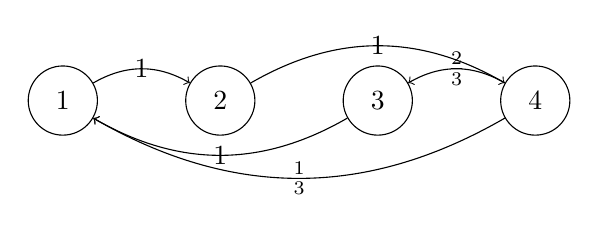
\begin{tikzpicture}[baseline={(current bounding box.center)}]
    %states
    \node[state] (2) at (-1,0) {$2$};
    \node[state] (3) at (1,0) {$3$};
    \node[state] (4) at (3,0) {$4$};
    \node[state] (1) at (-3,0) {$1$};
    %edges
    \path[->] 
%      (0) edge[loop above] node{$\frac{1}{3}$} (0)
     (1) edge[bend left] node{$1$} (2)
     (2) edge[bend left] node{$1$} (4)
     (3) edge[bend left] node{$1$} (1)
     (4) edge[bend left] node{$\frac{1}{3}$} (1)
     (4) edge[bend right] node{$\frac{2}{3}$} (3);
   \end{tikzpicture} 
\end{center}
From the graph, we can know $\big\{1,2,3,4\big\}$ is an irreducible set, state $2$ will come back in $3$ or $4$ steps, gcd is $1$, it is aperiodic, by Lemma 68, we can know all states are aperiodic as well, and by Theorem 66, we know the chain \textbf{can} converge to equilibrium.Use Matlab to calculate the left eigenvector and normalize, and $\pi P=\pi $ we can have\\
\begin{equation*}
    \pi(1)= .2727,\quad \pi(2)= .2727,\quad \pi(3)= .1818, \quad \pi(4)= .2727.
\end{equation*}
(c) \begin{center}
   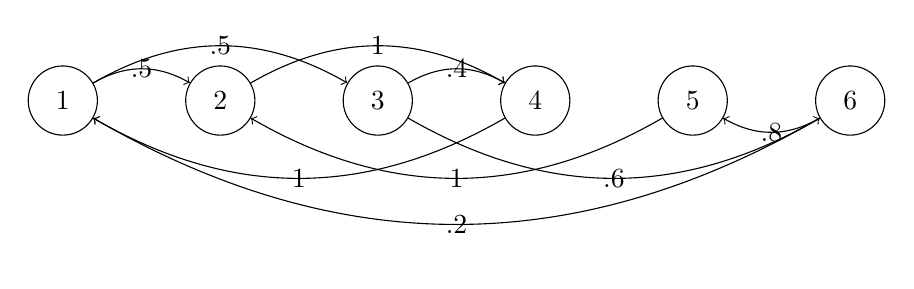
\begin{tikzpicture}[baseline={(current bounding box.center)}]
    %states
    \node[state] (6) at (5,0) {$6$};
    \node[state] (5) at (3,0) {$5$};
    \node[state] (4) at (1,0) {$4$};
    \node[state] (3) at (-1,0) {$3$};
    \node[state] (2) at (-3,0) {$2$};
    \node[state] (1) at (-5,0) {$1$};
    %edges
    \path[->] 
%      (0) edge[loop above] node{$\frac{1}{3}$} (0)
     (1) edge[bend left] node{$.5$} (2)
     (1) edge[bend left] node{$.5$} (3)
     (2) edge[bend left] node{$1$} (4)
     (3) edge[bend left] node{.4} (4)
     (3) edge[bend right] node{.6} (6)
     (4) edge[bend left] node{1} (1)
     (5) edge[bend left] node{1} (2)
     (6) edge[bend left] node{.2} (1)
     (6) edge[bend left] node{.8} (5);
   \end{tikzpicture} 
\end{center}
From the graph, we can know $\big\{1,2,3,4,5,6\big\}$ is an irreducible set, state $2$ is periodic, by Lemma 68, we can know all states are periodic with period $3$, thus, the chain \textbf{cannot} converge to equilibrium.\\
\end{itemize}

\pagebreak

\begin{itemize}
  \item 
\textbf{Exercise 1.17.}\\
Probability transition matrix, $S=\big\{0,1\big\}$, $0=$without cable, $1=$with cable:
\begin{align*}
P =\begin{array}{c} 0\\ 1 \end{array} \left( \begin{array}{ c c}
 0.74 & 0.26\\
 0.08 & 0.92 
\end{array}\right)
\end{align*}
We can use $P$ to predict the percentage in $1995$,
\begin{align*}
(0.436,0.564) P = (0.436,0.564)\left( \begin{array}{ c c}
 0.74 & 0.26\\
 0.08 & 0.92 
\end{array}\right)=(0.3678,0.6322)
\end{align*}
which is closed to the actual value $63.4\%$.\\
The percentage in $2000$,
\begin{align*}
(0.436,0.564) P^2 = (0.436,0.564)\left( \begin{array}{ c c}
 0.74 & 0.26\\
 0.08 & 0.92 
\end{array}\right)^2=(0.3227,0.6773)
\end{align*}
\begin{align*}
(0.366,0.634) P = (0.436,0.564)\left( \begin{array}{ c c}
 0.74 & 0.26\\
 0.08 & 0.92 
\end{array}\right)=(0.3216,0.6784)
\end{align*}
Both of these predictions are closed to actual percentage $68\%$. Since the chain is irreducible and aperiodic, we have limit distribution $(0.436,0.564)$ P^n, $\pi=\pi P$, use the formula of $2-$state MC
\begin{equation*}
    \pi = (\frac{0.08}{0.08+0.26},\frac{0.26}{0.08+0.26})=(\frac{4}{17},\frac{13}{17})
\end{equation*}
The long run proportion of people with cable is $\frac{13}{17}$.
\end{itemize}

\vspace{.1in}

\begin{enumerate}[\textbf{1.}]
  \item 
Exercise 1.8(c). \\
We know irreducible sets are $\big\{2,4\big\}$ and $\big\{1,5\big\}$, we can have transition matrix and stationary distribution as below
\begin{align*}
P_1 = \begin{array}{c} 2\\ 4 \end{array}\left( \begin{array}{ c c}
 0.2 & 0.8\\
 0.6 & 0.4 
\end{array}\right)
\end{align*}
\begin{align*}
P_2 = \begin{array}{c} 1\\ 5 \end{array}\left( \begin{array}{ c c}
 0 & 1\\
 0.3 & 0.7 
\end{array}\right)
\end{align*}
use $2-$state MC formula
\begin{equation*}
\begin{align*}
     (\frac{0.6}{0.6+0.8},&\frac{0.8}{0.6+0.8})=(\frac{3}{7},\frac{4}{7})\\
     \pi_1 =& (0,\frac{3}{7},0,\frac{4}{7},0)\\
    (\frac{0.3}{0.3+1},&\frac{1}{0.3+1})=(\frac{3}{13},\frac{10}{13})\\
    \pi_2 = &(\frac{3}{13},0,0,0,\frac{10}{13})
 \end{align*}
\end{equation*}
since $\alpha_1 +\alpha_2 =1$, $\alpha_1, \alpha_2 >0$
\begin{equation*}
    \pi = (\frac{3}{13}\alpha_2,\frac{3}{7}\alpha _1,0,\frac{4}{7}\alpha_1,\frac{10}{13}\alpha_2).
\end{equation*}
\end{enumerate}
\pagebreak

\vspace{.1in}

\begin{enumerate}[\textbf{2.}]
  \item
Since there exists $n \geq 1$ such that every entry of the $n-$step transition matrix $P^{n}$ is strictly positive (i.e. $p^{n}(x, y) > 0$ for all $x$, $y$), we can have 
\begin{equation*}
    p^{n+1}(x,y)= \sum_{z\in S}p^{n}(x,z)p(z,y)> p^{n}(x,z)p(z,y)>0
\end{equation*}
now, we can have $ p^{n+1}(x,x)>0$ and $ p^{n}(x,x)>0$,the period of x must divide $n$ and $n+1$, only $1$ meet this requirement, by Lemma $67$, we can say $x$ is aperiodic. Also, $p^{n}(x, y) > 0$ is equivalent to 
\begin{equation*}
    \rho_{xy} >0 \quad and \quad \rho_{yx} >0
\end{equation*}
then DTMC is irreducible, all states communicate with each other, thus, by Lemma 68, all states are aperiodic.
\end{enumerate}

\vspace{.1in}


\begin{enumerate}[\textbf{3.}]
  \item 
Draw a transition graph as below
\begin{center}
   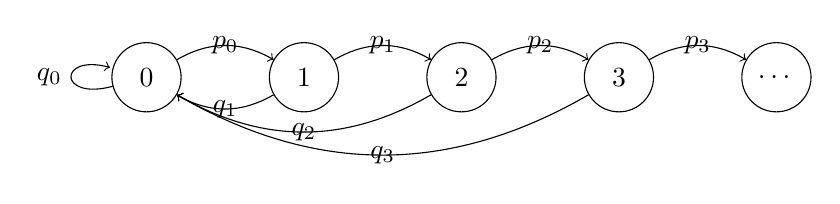
\begin{tikzpicture}[baseline={(current bounding box.center)}]
    %states
    \node[state] (1) at (-2,0) {$1$};
    \node[state] (2) at (0,0) {$2$};
    \node[state] (3) at (2,0) {$3$};
    \node[state] (0) at (-4,0) {$0$};
    \node[state] (upper) at (4,0) {$\dots$};
    %edges
    \path[->] 
%      (0) edge[loop above] node{$\frac{1}{3}$} (0)
     (0) edge[loop left] node{$q_0$} (0)
     (0) edge[bend left] node{$p_0$} (1)
     (1) edge[bend left] node{$p_1$} (2)
     (2) edge[bend left] node{$p_2$} (3)
     (3) edge[bend left] node{$p_3$} (upper)
     (2) edge[bend left] node{$q_2$} (0)
     (1) edge[bend left] node{$q_1$} (0)
     (3) edge[bend left] node{$q_3$} (0);
   \end{tikzpicture} 
\end{center}
We can see all states communicate with each other, if state $i$ is recurrent, then all states are recurrent, assume state $0$ is recurrent
\begin{equation*}
    P_0(T_{0} =\infty) = 0
\end{equation*}
$P_0(T_{0} =\infty) = p_0 p_1 p_2 p_3 ... $ holds, since
\begin{equation*}
\begin{align*}
       &p_0 p_1 p_2 p_3 ...\\
     = &\lim_{n\to\infty} p_0 p_1 p_2 p_3 ...p_n \\
     = &\lim_{n\to\infty}P_0(T_0 >n)\\
\end{align*}
\end{equation*}
 by continuity of probability measures with intersections\\
 \begin{equation*}
 \begin{align*}
     = &P(\bigcup\limits_{n=1}^{\infty } \big\{T_0 > n\big\})\\
     = &P_0(T_{0} =\infty)
\end{align*} 
 \end{equation*}   
then, we need to prove $p_0 p_1 p_2 p_3 ...=0$
\begin{equation*} 
\begin{align*}
       &\lim_{n\to\infty} p_0 p_1 p_2 p_3 ...p_n\\
     = & \prod_{n=1}^{\infty} \frac{2^n +1}{2^n +2}\to 0
\end{align*}
\end{equation*}
\begin{equation*} 
\begin{align*}
      P_0(T_{0} <\infty) = 1-P_0(T_{0} =\infty) = 1
\end{align*}
\end{equation*}
thus, all states are recurrent.
\end{enumerate}
\pagebreak

\begin{enumerate}[\textbf{4.}]
  \item 
(a) We can have 
\begin{equation*}
    P(Y<\infty ) = P(6^N <\infty )= P(N< \infty )
\end{equation*}
for proving $P(N< \infty) =1$, which means after finite time $N$, we will toss Head, we can draw a transition graph\\
\begin{center}
   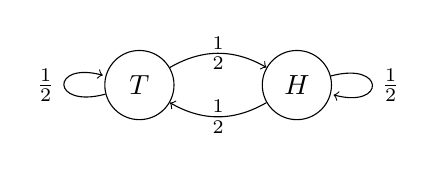
\begin{tikzpicture}[baseline={(current bounding box.center)}]
    %states
    \node[state] (H) at (1,0) {$H$};
    \node[state] (T) at (-1,0) {$T$};
    %edges
    \path[->] 
%      (0) edge[loop above] node{$\frac{1}{3}$} (0)
     (H) edge[loop right] node{$\frac{1}{2}$} (H)
     (T) edge[loop left] node{$\frac{1}{2}$} (T)
     (H) edge[bend left] node{$\frac{1}{2}$} (T)
     (T) edge[bend left] node{$\frac{1}{2}$} (H);
   \end{tikzpicture} 
\end{center}
we can know $\big\{T,H\big\}$ is irreducible, state $H$ and $T$ are recurrent. Then, assume we start from head 
\begin{equation*}
\begin{align*}
     P_H(T_H &< \infty) = 1 \\
     \big\{N<\infty \big\}&=\big\{T_H <\infty \big\}
\end{align*}
\end{equation*}
Thus, $P(Y<\infty ) =1$ holds.\\
Since
\begin{equation*}
\begin{align*}
   E[Y]=& \sum_{y=0}^{\infty } yP(Y=y)\\
       =& \sum_{n=0}^{\infty } 6^{n}P(N=n)\\
       =& \sum_{n=0}^{\infty } 6^{n}\frac{1}{2}^{n}\\
       =& \sum_{n=0}^{\infty } 3^{n} \to\ \infty 
\end{align*}   
\end{equation*}
$E[Y] = \infty $ holds.\\
\\
(b) Running those codes in Matlab, result as below\\
$N=3$, $Y=216$\\
\\
(c)(d) Running those codes in Matlab, plots showed \textbf{in the last page}.\\
\begin{figure}[h!]
\begin{align*}
\includegraphics[scale=.2]{untitled1.jpg}
\includegraphics[scale=.2]{p2.jpg}\\
\includegraphics[scale=.2]{p3.jpg}
\includegraphics[scale=.2]{p4.jpg}\\
\includegraphics[scale=.2]{p5.jpg}
\includegraphics[scale=.2]{p6.jpg}
\end{align*}
\end{figure}

\\
 $A(m)$ will \textbf{not} converge for $m$ going to infinity. From plots, we can see $A(m)$ fluctuates, after merging to a higher point, it will go down. Given $A(m) = \frac{1}{m}\sum_{i=1}^{m}Y(i)$, we know the merge happen resulting from the value of $Y(i)$ is large based on running above codes, the decrease come with $m$ increase, thus, $A(m)$ will not converge.  
\end{enumerate}
\end{document}
